% Provenance (never printed): see sources/outline_sources.md (Year 3: gravity, magnetic,
% seismic, resistivity and ground-penetrating-radar surveys; data processing and
% uncertainty; a mapping project).
% Brief: sources/book5/BRIEFS.md, ch. 31. Curves from figdata/bachelor-3/gravity_granite.py
% (prism model of the Varden granite of figdata/shared/region.py), magnetic_dyke.py (2-D
% dyke; the Varden dolerite dyke of the Sync 3 ruling, buried below the unconformity),
% resistivity_sounding.py (Pekeris transform and image series) and gpr_radargram.py.
% Physical-property ranges and survey practice from the GPG open textbook (CC BY 4.0) and
% Keys (1990). Exercise and problem values in the Book 5 scratch calculator calc/ch31.py.
\chapter{طرائق الحقل والمختبر III}\label{ch:b3:field-lab-methods-3}

يقضي فريق جيوفيزيائي أسبوعًا في وادي تلال فاردن،
المنطقة المتخيّلة التي رسم مجلد السنة الأولى خريطتها الجيولوجية في
فصله عن الخرائط الجيولوجية. تُظهر الخريطة جرانيتًا ظاهرًا على
جانبي الوادي، بين الشيست، تحت الحجر الرملي الذي يرتكز على
كليهما. أمّا أين يغوص الجرانيت تحت الغطاء وإلى أي مدى يمتد
وإلى أي عمق يصل، فلم يشاهده أحد. يحمل الفريق
مقياس جاذبية، ومقياسي مغناطيسية، وكبلًا من الأقطاب ورادارًا على
عربة صغيرة. لا يرى أيٌّ من هذه الأجهزة صخرًا: كلّ منها يقيس
حقلًا عند السطح---الجاذبية، والحقل المغناطيسي، وكمونًا كهربائيًا،
وصدى نبضة راديوية---وهي حقول تُخلّ بها الصخور الواقعة تحتها.
بنهاية الأسبوع يستطيع الفريق أن يرسم الجرانيت الذي لم يرَه قط، وأن يقول
كم يبلغ عمق الرواسب الغرينية في قاع الوادي، وأن يُبلغ عن جسم مغناطيسي
لم تُظهره أي خريطة.

يتتبّع هذا الفصل ذلك الأسبوع. يعالج كل طريقة على حدة، بوصفها قياسًا مع تصحيحاته،
وبوصفها مسألة مباشرة ذات أجسام قليلة يمكن حساب حقولها بدقة؛
ثم يبيّن كيف تتراكم أخطاء المسح، ولماذا
نادرًا ما يحدّد نوعٌ واحد من البيانات نموذجًا بعينه؛ ويختم بمسح تلال فاردن، حيث توضع
الطرائق
معًا.

\begin{recall}
شذوذ الجاذبية، وتصحيحا الهواء الحرّ وبوغير وشذوذاهما،
والجاذبية المرجعية، واردة في مجلد السنة الأولى، في فصله عن التوازن الأيزوستاتي
والجاذبية؛ ودورة المسح \omterm{def:b3:field-lab-methods-3:gravimeter}{لمقياس الجاذبية النسبي} موصوفة في
\cref{ch:b3:gravity-geodesy}. يرد الحقل الرئيسي وميله، \omterm{thm:b3:palaeomagnetism:dipole}{وصيغة
ثنائي القطب}، \omterm{def:b3:palaeomagnetism:igrf}{والمجال المغناطيسي الأرضي المرجعي الدولي} موجودة في
\cref{ch:b3:palaeomagnetism}. والمقاومية وقانون أوم والسماحية النسبية
والموجات الكهرطيسية والمغنطة والقابلية المغناطيسية واردة في كتب الفيزياء،
ومبرهنة غاوس للجاذبية معها.
\omterm{def:b3:exploration-seismology:surveys}{المسح الزلزالي الانكساري} موجود في
\cref{ch:b3:exploration-seismology}؛ \omterm{def:b3:seismology-imaging:inverse}{المسألة المباشرة} \omterm{def:b3:seismology-imaging:inverse}{والمسألة العكسية} والمربعات
الصغرى الموزونة في \cref{ch:b3:seismology-imaging}؛ والمسامية في
كتب المدرسة، وسجلّات الآبار السلكية في \cref{ch:b3:facies-models}. ويرد
انتشار عدم اليقين في كتب الكيمياء والرياضيات.
\end{recall}

\section{مسوح الجاذبية}\label{sec:b3:field-lab-methods-3:gravity}

الشذوذات التي يبحث عنها مسح الجاذبية صغيرة. تبلغ الجاذبية عند
خط الاستواء نحو \qty{978000}{\milli\gal}؛ وتُغيّرها البنى الكبيرة
بمئات المليغال، والقبة الملحية بنحو عشرة، والجسم المعدني بنحو
واحد، وأهداف المسح الجيوتقني بعدة
أجزاء من المئة. يقيس الجيوفيزيائيون بالمليغال،
أو بوحدات جاذبية قدرها \qty{0.1}{\milli\gal}؛ ويجب أن يميّز المسح المفيد
الفروق بمقدار جزء واحد من مئة مليون من~$g$.
% ledger: gpg:grav-units, gpg:grav-sizes

\begin{definition}[مقياس الجاذبية النسبي؛ الانجراف الآلي]\label{def:b3:field-lab-methods-3:gravimeter}
\emph{مقياس الجاذبية النسبي}\index{مقياس الجاذبية النسبي} هو
جهاز يقيس فروق الجاذبية بين المحطات: كتلة
معلّقة بنابض، تُحفظ عند وضع الصفر بقوة ثانية قابلة للضبط
يُعطي قراءة مؤشّرها، مضروبةً في ثابت معايرة، الجاذبية
بالمليغال حتى ثابت مجهول. ويُسمّى \emph{
الانجراف الآلي}\index{الانجراف الآلي} التغيّر البطيء لقراءته عند
محطة ثابتة، ناتج عن زحف النابض والحرارة والصدمات؛ ويُقاس
بإعادة القراءة بعد بضع ساعات في محطة سبق قراءتها،
وهي \emph{محطة الأساس}.
\end{definition}
% ledger: gpg:gravimeter, gpg:grav-survey

يغطي مقياس الجاذبية الحقلي مدًى يبلغ عشرات الآلاف من
المليغالات، ويقرأ في أفضل حالاته حتى نحو \qty{0.01}{\milli\gal}؛ ويجب
إعادة ضبط المدى بعد النقل. وعند هذه الدقة تكون ارتفاعات
المحطات بأهمية قراءتها: فخطأ ارتفاع قدره \qty{3.3}{cm}
يُفسد \qty{0.01}{\milli\gal}، لذلك تُمسح المواقع بأجهزة استقبال
الأقمار الصناعية أو بالميزان حتى السنتيمتر. وتُعاد زيارة محطة الأساس
كل ساعتين تقريبًا. ويتغيّر المدّ الأرضي الصلب، الذي يمكن أن يبلغ
\qty{0.3}{\milli\gal}، ببطء كافٍ خلال تلك الساعات حتى يمكن
إزالته مع الانجراف.
% ledger: gpg:gravimeter, gpg:grav-survey, gpg:grav-sizes

\begin{method}[اختزال دورة الجاذبية]\label{met:b3:field-lab-methods-3:loop}
تبدأ الدورة وتنتهي عند محطة أساس، تُقرأ في الزمنين $t_0$ و$t_1$.
\begin{enumerate}
  \item احسب معدّل الانجراف $(r_1 - r_0)/(t_1 - t_0)$ من القراءتين
        عند محطة الأساس؛ ويتضمّن المدّ.
  \item اطرح من كل قراءة الانجراف المتراكم منذ $t_0$،
        $r - (t - t_0)(r_1 - r_0)/(t_1 - t_0)$، واطرح قراءة الأساس
        فتكون الجاذبية نسبةً إلى محطة الأساس.
  \item صحّح الارتفاع $\Delta h$ للمحطة فوق محطة الأساس:
        أضف تصحيح الهواء الحرّ $\qty{0.3086}{\milli\gal.m^{-1}}
        \times\Delta h$ واطرح تصحيح بوغير
        $\qty{0.1119}{\milli\gal.m^{-1}}\times\Delta h$ (الكثافة
        \qty{2670}{kg.m^{-3}})، أي أضف $0.1967\,\Delta h$.
  \item لمحطة تبعد مسافة $\Delta y$ شمال محطة الأساس، اطرح
        تغيّر الجاذبية المرجعية، $\qty{0.811}{\milli\gal.km^{-1}}
        \times\sin 2\varphi\times\Delta y$.
  \item أضف \omterm{def:b3:field-lab-methods-3:terrain}{تصحيح التضاريس} لكل محطة.
\end{enumerate}
والنتيجة هي شذوذ بوغير نسبةً إلى محطة الأساس. وبربط محطة الأساس
بمحطة ذات جاذبية مطلقة معلومة يُعطى الشذوذ نفسه.
\end{method}
% ledger: gpg:grav-survey, gpg:terrain

يعامل تصحيح بوغير الأرض الواقعة بين المحطة ومستوى
المرجع كأنها لوح مستوٍ. وفي تضاريس حقيقية يكون هذا خاطئًا مرتين:
فتلّة ترتفع فوق المحطة تجذب إلى أعلى فتُخفض
القراءة، ووادٍ ينخفض دونها يُحسب في اللوح على أنه
صخرٌ غير موجود.

\begin{definition}[تصحيح التضاريس]\label{def:b3:field-lab-methods-3:terrain}
\emph{تصحيح التضاريس}\index{تصحيح التضاريس} لمحطة الجاذبية هو الجذب الذي
تمارسه انحرافات التضاريس عن لوح بوغير على المحطة: التلالُ فوق مستوى المحطة،
والأودية تحتها، محسوبةً بكثافة اللوح.
وكلاهما يُخفض الجاذبيةَ المقيسةَ قياسًا على اللوح،
لذا يُضاف التصحيح
دائمًا.
\end{definition}

كان يُحسب يدويًا بمخطط هامر وجداول، منطقةً فمنطقةً
بالابتعاد عن المحطة؛ ويُحسب اليوم من نموذج الارتفاع الرقمي.
وبعيدًا عن التضاريس الحادة نادرًا ما يتجاوز \qty{1}{\milli\gal}،
لكنّ المناطق القريبة من المحطة يصعب ضبطها بدقّة،
ولا يُعرف التصحيح عادةً بدقة أفضل من \qty{0.2}{\milli\gal}.
% ledger: gpg:terrain, gpg:grav-sizes

\subsection{شذوذ الأجسام البسيطة}

\omterm{def:b3:seismology-imaging:inverse}{المسألة المباشرة} للجاذبية مجموعٌ: يجذب كلُّ عنصرٍ من جسمٍ ذي
تباينِ كثافةٍ $\Delta\rho$ المحطةَ وفق قانون نيوتن، ويقيس المسحُ
المركبةَ الرأسية للمجموع. وتُعطي أجسامٌ قليلةٌ
ذلك في صورة مغلقة.

\begin{theorem}[الكرة والأسطوانة الأفقية]\label{thm:b3:field-lab-methods-3:sphere}
عند مسافة أفقية $x$ عن النقطة الواقعة فوق مركزها، تُعطي كرةٌ مدفونةٌ
ذاتُ كتلةٍ زائدةٍ $\Delta m$ ومركزُها على عمق $z$
الشذوذَ الآتي:
\[
\Delta g(x) = \frac{G\,\Delta m\,z}{(x^2 + z^2)^{3/2}} ,
\]
ويهبط الشذوذ إلى نصف قمّته عند $x_{1/2} = z\sqrt{2^{2/3} - 1}$،
بحيث يكون $z = 1.305\,x_{1/2}$. وتُعطي أسطوانةٌ أفقيةٌ طويلةٌ ذاتُ كتلةٍ زائدةٍ
$\lambda$ لكل وحدة طول، ومحورُها على عمق $z$، يُعطي عبر
امتدادها الشذوذَ الآتي:
\[
\Delta g(x) = \frac{2G\lambda z}{x^2 + z^2} ,
\]
و$z = x_{1/2}$.
\end{theorem}

\begin{proof}
خارج كرةٍ تتعلّق كثافتُها بالبعد عن مركزها وحده،
تكون الجاذبيةُ جاذبيةَ كتلتِها الموضوعةَ في المركز (مبرهنةُ
القشرة، وهي نتيجة لمبرهنة غاوس). ومقدارُ الجاذبية عند
المحطة هو $G\Delta m/(x^2 + z^2)$، وتحمل المركبةُ الرأسية
العاملَ $z/\sqrt{x^2 + z^2}$. وبكتابة $\Delta g(x_{1/2}) =
\Delta g(0)/2$ نحصل على $(1 + x_{1/2}^2/z^2)^{3/2} = 2$، ومنه القاعدةُ. أمّا
بالنسبة للأسطوانة فتُعطي مبرهنةُ غاوس على أسطوانة متحدةِ المحور نصفُ قطرها $r$
مجالًا قدره $2G\lambda/r$، والمركبةُ الرأسية $2G\lambda z/r^2$؛
ويُبلغ نصفُ القمة عندما $x^2 + z^2 = 2z^2$.
\end{proof}
% ledger: gpg:half-width

للجسم غير الكروي عرضٌ عند نصف القمة أيضًا، وتُعطي القاعدةُ حينئذٍ
عمقَ كرةٍ مكافئةٍ لا عمقَ الجسم نفسه. والقاعدةُ
تقديرٌ أوليّ يُجرى قبل ملاءمة أيّ نموذج.

\begin{proposition}[الأسطوانة الرأسية على محورها]\label{prop:b3:field-lab-methods-3:vcyl}
أسطوانةٌ رأسية نصف قطرها $a$ وتباين كثافتها $\Delta\rho$،
وقمّتُها وقاعدتُها على عمقَي $z_1 < z_2$ تحت المحطة، تُعطي
على محورها
\[
\Delta g = 2\pi G\Delta\rho\left[(z_2 - z_1) + \sqrt{z_1^2 + a^2}
           - \sqrt{z_2^2 + a^2}\right] .
\]
وعندما $a \to \infty$ يكون هو لوح بوغير $2\pi G\Delta\rho(z_2 - z_1)$؛
أمّا الأسطوانة الممتدةُ من السطح إلى عمق كبير فتؤول إلى
$2\pi G\Delta\rho\,a$.
\end{proposition}

\begin{proof}
قرصٌ نصف قطره $a$ وسمكُه $\mathrm{d}z$ على عمق $z$ يجذب
نقطةً على محوره بمقدار $2\pi G\Delta\rho\,\mathrm{d}z\,(1 -
z/\sqrt{z^2 + a^2})$، وهو جذب حلقةٍ مكاملٌ
على نصف القطر. وبالتكامل من $z_1$ إلى $z_2$ نحصل على القوس. وعندما $a \to
\infty$ مع ثبات العمقين، $\sqrt{z_1^2 + a^2} - \sqrt{z_2^2 + a^2} =
(z_1^2 - z_2^2)/(\sqrt{z_1^2 + a^2} + \sqrt{z_2^2 + a^2}) \to 0$؛ وعندما
$z_1 = 0$ و$z_2 \to \infty$، $z_2 - \sqrt{z_2^2 + a^2} \to 0$
ويؤول القوس إلى $a$.
\end{proof}

\begin{proposition}[الكتلة الزائدة من خريطة الجاذبية]\label{prop:b3:field-lab-methods-3:gauss}
مهما كان شكلُ جسمٍ يقع بكامله تحت مستوٍ أفقي،
فإنّ كتلتَه الزائدةَ هي
\[
\Delta m = \frac{1}{2\pi G}\iint \Delta g\,\mathrm{d}A ,
\]
حيث يشمل التكامل المستوى كلّه.
\end{proposition}

\begin{proof}
بالنسبة لكتلة نقطية $m$ على عمق $z$، و$r$ المسافة الأفقية،
$\iint \Delta g\,\mathrm{d}A = \int_0^\infty
Gmz\,(r^2 + z^2)^{-3/2}\,2\pi r\,\mathrm{d}r = 2\pi Gm$: نصفُ التدفق
$4\pi Gm$ لمبرهنة غاوس يعبر المستوى. ويُعدّ الجسم مجموعًا لكتل نقطية،
والتكامل خطيٌّ.
\end{proof}

تُعطي المبرهنةُ الكتلةَ لا الشكلَ أبدًا؛ والخريطةُ لا تغطي إلا جزءًا من
المستوى، بينما يتناقص شذوذُ الجسم العميق ببطء، فتكون
الكتلة المستخلصة من الخريطة أصغرَ من الحقيقة ما لم تُمدّ حوافُّه
بنموذج.

\begin{omfigure}
\begin{tikzpicture}
\begin{axis}[axis equal image, xmin=1.5, xmax=5.5, ymin=2.6, ymax=5.7, width=0.86\linewidth,
  tick label style={font=\scriptsize}, xlabel={شرق \babelsublr{(km)}}, ylabel={شمال \babelsublr{(km)}},
  label style={font=\small}, unbounded coords=jump]
% geology of the region (figdata/shared/region.py), faded
\addplot[lith schist, draw=black!50, line width=0.2pt, even odd rule, opacity=0.45] table {figdata/out/shared-region-unit-schist.dat};
\addplot[lith granite, draw=black!50, line width=0.2pt, even odd rule, opacity=0.45] table {figdata/out/shared-region-unit-granite.dat};
\addplot[om lith={icsTriassic!35}{om sand}, draw=black!50, line width=0.2pt, even odd rule, opacity=0.45] table {figdata/out/shared-region-unit-sandstone.dat};
\addplot[om lith={icsJurassic!40}{om limestone}, draw=black!50, line width=0.2pt, even odd rule, opacity=0.45] table {figdata/out/shared-region-unit-limestone.dat};
\addplot[om lith={icsJurassic!15}{om shale}, draw=black!50, line width=0.2pt, even odd rule, opacity=0.45] table {figdata/out/shared-region-unit-shale.dat};
\addplot[lith alluvium, draw=black!50, line width=0.2pt, even odd rule, opacity=0.45] table {figdata/out/shared-region-unit-alluvium.dat};
\addplot[river] table {figdata/out/shared-region-river.dat};
% the survey (figdata/bachelor-3/gravity_granite.py, magnetic_dyke.py)
\addplot[only marks, mark=*, mark size=0.7pt, black!70] table[x=x_km, y=y_km] {figdata/out/bachelor-3-gravity_granite-stations.dat};
\addplot[omDef, very thick] table[x=x_km, y=y_km] {figdata/out/bachelor-3-gravity_granite-contours.dat};
\addplot[omThm, thick] coordinates {(1.5,4.15) (5.5,4.15)};
\addplot[omMeth, line width=2.2pt, opacity=0.8] coordinates {(1.7,4.15) (2.7,4.15)};
\addplot[omProp, dashed, thick] coordinates {(2.2,2.6) (2.2,5.7)};
\addplot[only marks, mark=star, mark size=3.5pt, omMeth!70!black, thick] coordinates {(3.5,4.0)};
\node[font=\scriptsize, fill=white, fill opacity=0.85, text opacity=1, inner sep=1pt] at (axis cs:3.5,5.12) {$-0.5$};
\node[font=\scriptsize, fill=white, fill opacity=0.85, text opacity=1, inner sep=1pt] at (axis cs:3.5,4.84) {$-1$};
\node[font=\scriptsize, fill=white, fill opacity=0.85, text opacity=1, inner sep=1pt] at (axis cs:3.5,4.58) {$-2$};
\node[font=\scriptsize, anchor=south west, fill=white, fill opacity=0.85, text opacity=1, inner sep=1pt] at (axis cs:1.55,4.17) {مقطع الجاذبية};
\node[font=\scriptsize, anchor=north, fill=white, fill opacity=0.85, text opacity=1, inner sep=1pt] at (axis cs:2.2,4.08) {الخط المغناطيسي};
\node[font=\scriptsize, anchor=north west, text=omProp!80!black, fill=white, fill opacity=0.85, text opacity=1, inner sep=1pt] at (axis cs:2.24,5.6) {قاطع مدفون};
\node[font=\scriptsize, anchor=north, fill=white, fill opacity=0.85, text opacity=1, inner sep=1pt] at (axis cs:3.5,3.92) {السبر};
\pic at (axis cs:5.15,5.3) {northarrow};
\end{axis}
\end{tikzpicture}

\par\smallskip{\small مسح فاردن فوق الخريطة الجيولوجية للمنطقة
(باهتة: الشيست رمادي، الجرانيت وردي، الحجر الرملي والحجر الجيري والطَّفل من
الغطاء، والطمي على امتداد النهر). نقاط سوداء: محطات الجاذبية،
\qty{200}{m} تفصل بينها؛ أزرق: شذوذ بوغير لنموذج الجرانيت،
مرسومًا بخطوط كنتورية كل \qty{0.5}{\milli\gal}؛ أحمر: مقطع الجاذبية؛ أخضر:
الخط المغناطيسي والسبر الكهربائي (النجمة) على قاع الوادي؛
 برتقالي متقطّع: القاطع الدولوريتي الذي يكشفه المسح المغناطيسي،
المدفون تحت الغطاء.}\label{fig:b3:field-lab-methods-3:survey}
\end{omfigure}
% ledger: gpg:densities

\subsection{جرانيت فاردن}

يُعدّ نموذج الجيولوجيين للجرانيت جسمًا ناقصيًّا يقع أسفل عدم التوافق،
بعرض \qty{760}{m} من الشرق إلى الغرب و\qty{1120}{m}
من الشمال إلى الجنوب عند التقائه بالغطاء، ويتّسع نحو الأسفل؛ أمّا على
جانبي الوادي فيصل إلى السطح. الجرانيت أخفّ من الشيست:
تقع مديات الكثافة المنشورة في \numrange{2.50}{2.81}
و\qtyrange{2.39}{2.80}{g.cm^{-3}}. ويأخذ نموذج المسح
\qty{2620}{kg.m^{-3}} للجرانيت و\qty{2750}{kg.m^{-3}} للشيست،
بتباين قدره \qty{-130}{kg.m^{-3}}، ويُوقف الجرانيت عند
عمق \qty{1500}{m} تحت مستوى سطح البحر، وهذا افتراض لأنّ لا شيء يُظهر
قاعَه. يُقسَّم إلى \num{5533} منشورًا قائمًا جواذبها ذات صيغة مغلقة،
فيُعطي النموذج شذوذ الخريطة أعلاه: انخفاضًا مغلقًا قدره
\qty{-2.29}{\milli\gal} فوق مركز الجرانيت، وتمتدّ خطوطه الكنتورية
ممتدّة من الشمال إلى الجنوب شبهًا بالجسم.
% ledger: gpg:densities

\begin{omfigure}
\begin{tikzpicture}
\begin{axis}[width=0.8\linewidth, height=0.42\linewidth, xmin=1.5, xmax=5.5, ymin=-2.6, ymax=0.2,
  xlabel={الشرق \babelsublr{(\unit{km})}}, ylabel={الشذوذ $\Delta g$ \babelsublr{(\unit{\milli\gal})}},
  tick label style={font=\scriptsize}, label style={font=\small},
  legend style={font=\scriptsize, at={(0.02,0.04)}, anchor=south west}]
% computed in figdata/bachelor-3/gravity_granite.py
\addplot[omDef, very thick] table[x=x_km, y=dg_mGal] {figdata/out/bachelor-3-gravity_granite-profile.dat};
\addlegendentry{نموذج الجرانيت}
\addplot[omThm, densely dashed, thick] table[x=x_km, y=sphere] {figdata/out/bachelor-3-gravity_granite-profile.dat};
\addlegendentry{الكرة وفق قاعدة نصف العرض}
\addplot[omMeth, densely dotted, thick] table[x=x_km, y=cyl] {figdata/out/bachelor-3-gravity_granite-profile.dat};
\addlegendentry{أسطوانة رأسية}
\addplot[black!40, forget plot] coordinates {(1.5,0) (5.5,0)};
\addplot[black!50, densely dotted, forget plot] coordinates {(1.5,-1.1464) (5.5,-1.1464)};
\node[font=\scriptsize, black!60, anchor=south east] at (axis cs:5.45,-1.14) {نصف الذروة};
\end{axis}
\end{tikzpicture}

\par\smallskip{\small الشذوذ على امتداد مقطع الجاذبية (الأزرق)، والكرة
التي تعطي قاعدة نصف العرض عمقها وكتلتها (أحمر متقطّع)،
وأسطوانة رأسية بالمساحة نفسها للجرانيت عند عدم التوافق،
من سطح الأرض إلى قاع النموذج (أخضر منقّط). تطابق الكرة
الذروة ونصف العرض بحكم البناء، لكنّها لا تطابق الجوانب؛ أمّا
الأسطوانة، التي تتجاهل اتّساع الجسم، فتقصر عند
المركز.}\label{fig:b3:field-lab-methods-3:profile}
\end{omfigure}
% ledger: gpg:half-width

\section{المسوح المغناطيسية}\label{sec:b3:field-lab-methods-3:magnetics}

يبلغ المجال الرئيسي للأرض نحو \qty{25000}{nT} عند خطّ الاستواء المغناطيسي
ونحو \qty{70000}{nT} قرب القطبين المغناطيسيين. الصخور التي تحوي
المغنتيت تضيف إليه مجالها الخاصّ، المُستحَثّ بالمجال الرئيسي بنسبة
إلى قابليتها المغناطيسية، أو المغنطة المتبقّية المحمولة منذ الزمن
الذي تكوّنت فيه. للصخر الناري الفلسي قابلية مغناطيسية أقلّ من نحو
\num{2e-3}، أمّا المافي فيتراوح من نحو \num{2e-3} إلى \num{0.4}؛ وعلى المقياس
نفسه، تعطي واحد بالمئة من المغنتيت بالحجم نحو \num{0.03}.
% ledger: gpg:mag-field, gpg:susceptibility

\begin{definition}[شذوذ المجال الكلي؛ التصحيح اليومي؛ الاختزال إلى القطب]\label{def:b3:field-lab-methods-3:magnetic}
ليكن $\mathbf{F}$ المجال الرئيسي عند المسح و$\Delta\mathbf{B}$
مجال الصخور المُمغنطة.
  \begin{itemize}
  \item \emph{شذوذ المجال الكلي}\index{شذوذ المجال الكلي} هو
        الشدّة المقاسة مطروحًا منها شدّة المجال الرئيسي، $\Delta T =
        |\mathbf{F} + \Delta\mathbf{B}| - |\mathbf{F}|$؛ عندما
        $|\Delta\mathbf{B}| \ll |\mathbf{F}|$ فهو الإسقاط
        $\Delta\mathbf{B}\cdot\mathbf{F}/|\mathbf{F}|$.
  \item \emph{التصحيح اليومي}\index{التصحيح اليومي} يزيل
        تغيّرات المجال مع الزمن: يسجّل مقياس المغناطيسية عند محطة قاعدة
        ثابتة المجالَ طوال المسح، وكلّ
        قراءة $T(t)$ للجهاز المتحرّك تُستبدل بالقيمة $T(t) -
        T_\mathrm{base}(t)$.
  \item \emph{الاختزال إلى القطب}\index{الاختزال إلى القطب}
        يحسب، انطلاقًا من الشذوذ المقاس، الشذوذ الذي تعطيه الصخور نفسها
        لو كان المجال الرئيسي رأسيًا، كما هو عند قطب مغناطيسي،
        فيقع الشذوذ عندئذٍ فوق مصدره.
  \end{itemize}
\end{definition}
% ledger: gpg:mag-survey, gpg:mag-processing

تنشأ التغيّرات الزمنية عن تيّارات في الغلاف الأيوني، على ارتفاع نحو
\qty{110}{km} فوق سطح الأرض. وتبلغ هذه التغيّرات في اليوم عادةً ما يتراوح
من \qtyrange{20}{50}{nT}، أي بقدر شذوذ هدف صغير؛ وقد تُغيّر العاصفة
المغناطيسية المجال بآلاف النانوتسلا.
تقيس محطة القاعدة التغيّر، على افتراض أنّه
هو نفسه على امتداد المسح كلّه. ويُزال المجال الرئيسي نفسه، أو مجال
البنى الأكبر من مساحة المسح، باستخدام IGRF، بوصفه ثابتًا
أو اتّجاهًا مُلاءَمًا.
% ledger: gpg:mag-field, gpg:mag-processing

يقيس مقياس المغناطيسية ذو تقدّم البروتونات التردّدَ الذي يتقدّم عنده
دوران البروتونات في المجال، وهو متناسب مع المجال؛ ويقرأ بدقّة
\qty{1}{nT} ويحتاج إلى أكثر من ثانية لكلّ قراءة. أمّا
ويُعدّ مقياس المغناطيسية بالسيزيوم المُضَخّ ضوئيًا أكثر حساسيةً بعشر
إلى مئة مرّة، ويقرأ بدقّة \qty{0.01}{nT}. ويجب أن تكون المحطّات
متقاربةً بما يكفي لوضع ما لا يقل عن نحو ثلاث قراءات عبر نصف عرض
أضيقِ شذوذ يُبحث عنه، وكلّما كان المصدر أقرب إلى السطح وجب أن تكون
المحطّات أكثر تقاربًا.
% ledger: gpg:mag-survey

\begin{proposition}[شذوذ قاطع رفيع]\label{prop:b3:field-lab-methods-3:dyke}
قاطعٌ رأسي سمكه $t$ وقابليته المغناطيسية $\kappa$، يمتدّ
على طول خط الزوال المغناطيسي، وقمّته عند عمق $z$، ويمتدّ
إلى الأسفل بعيدًا، ممغنطًا بالحثّ في مجال رئيسي $F$ ذي ميل $I$،
فيعطي عبر امتداده، إذا كان $t \ll z$،
\[
\Delta T(x) = \frac{\kappa F t\sin^2 I}{2\pi}\,\frac{z}{x^2 + z^2} ,
\]
شذوذًا متناظرًا يهبط إلى نصف قمّته عند $x = \pm z$: العمق
إلى قمّة القاطع يساوي نصف العرض الكامل للشذوذ عند
نصف قمّته.
\end{proposition}

\begin{proof}
القاطع ثنائيّ البعد، والمجال الرئيسي يقع في المستوي الرأسي
للامتداد. أمّا المغنطة $\mathbf{M} = \kappa\mathbf{F}/\mu_0$
لها مركّبة على طول الامتداد، وأقطابها تقع عند طرفَي
القاطع بعيدًا، ولا تولّد حقلًا؛ ومركّبة رأسية $M
\sin I$، تضع على الوجه العلوي للقاطع شحنةً مغناطيسيةً
$-Mt\sin I$ لكلّ وحدة طول (حيث $\mathbf{M}\cdot\mathbf{n}$ هي
كثافة الشحنة، و$\mathbf{n}$ العمودي الخارجي)، والوجه السفلي
بعيد. تولّد شحنة خطية $q$ لكلّ وحدة طول، بحسب مبرهنة غاوس
في بعدين، حقلًا $q/(2\pi r)$ على طول نصف القطر. وعند
محطّة $(x, 0)$ فوق قمّة عند $(0, z)$ تكون مركّبتها الهابطة
$Mt\sin I\,z/(2\pi(x^2 + z^2))$، ومركّبتها الأفقية
عبر الامتداد، عمودية على $\mathbf{F}$. نضرب في
$\mu_0$ ونسقط على $\mathbf{F}$ التي مركّبتها الرأسية
$\sin I$، فنحصل على $\Delta T$. وشرط نصف القمّة هو $x^2 + z^2 =
2z^2$.
\end{proof}

عندما يمتدّ القاطع عبر خط الزوال، تقع الأجزاء الأفقية من
المغنطة والمجال الرئيسي كلاهما في مستوي
المقطع، فتحمل الأوجه الجانبية شحنات، ويصبح الشذوذ
غير متناظر، مع انخفاض على جهة القطب. ويحسب الشكل أدناه
ذلك بدقّة لقاطع ذي عرض منتهٍ، بجمع الحقول المغلقة
لأوجهه الأربعة المشحونة. ويُحوِّل \omterm{def:b3:field-lab-methods-3:magnetic}{الاختزال إلى القطب} هذا
الشذوذ إلى الشذوذ المتناظر لحقل رأسي.

\begin{omfigure}
\begin{tikzpicture}
\begin{groupplot}[group style={group size=2 by 1, horizontal sep=1.5cm},
  width=0.48\linewidth, height=0.42\linewidth,
  tick label style={font=\scriptsize}, label style={font=\small}, title style={font=\small}]
\nextgroupplot[xmin=-600, xmax=600, ymin=-6, ymax=28, xlabel={المسافة \babelsublr{(\unit{m})}},
  ylabel={\mbox{\textdir TLT $\Delta T$ (\unit{nT})}}, title={قاطع عند ميلين مختلفين},
  scaled x ticks=false,
  legend style={font=\scriptsize, at={(0.98,0.98)}, anchor=north east}]
% computed in figdata/bachelor-3/magnetic_dyke.py
\addplot[omDef, very thick] table[x=x_m, y=dT_I90] {figdata/out/bachelor-3-magnetic_dyke-generic.dat};
\addlegendentry{$I = 90^\circ$}
\addplot[omThm, thick] table[x=x_m, y=dT_I60] {figdata/out/bachelor-3-magnetic_dyke-generic.dat};
\addlegendentry{{\foreignlanguage{arabic}{\mbox{\textdir TLT $60^\circ$}، امتداد شرق--غرب}}}
\addplot[omMeth, densely dashed, thick] table[x=x_m, y=dT_I60ns] {figdata/out/bachelor-3-magnetic_dyke-generic.dat};
\addlegendentry{{\foreignlanguage{arabic}{\mbox{\textdir TLT $60^\circ$}، امتداد شمال--جنوب}}}
\addplot[black!40, forget plot] coordinates {(-600,0) (600,0)};
\node[font=\scriptsize, black!60, anchor=south west] at (axis cs:-590,-5.6) {جنوب};
\node[font=\scriptsize, black!60, anchor=south east] at (axis cs:590,-5.6) {شمال};
\nextgroupplot[xmin=1.7, xmax=2.7, ymin=0, ymax=40, xlabel={الشرق \babelsublr{(\unit{km})}},
  ylabel={الحقل $- \qty{48000}{nT}$}, title={خطّ فاردن كما قُرئ},
  legend style={font=\scriptsize, at={(0.02,0.98)}, anchor=north west}]
\addplot[omDef, thick, mark=*, mark size=1.1pt] table[x=x_km, y expr=\thisrow{T_obs}-48000] {figdata/out/bachelor-3-magnetic_dyke-line.dat};
\addlegendentry{الجهاز المتحرّك}
\addplot[omThm, thick, densely dashed] table[x expr=1.7+\thisrow{t_min}/40, y expr=\thisrow{T_base}-48000] {figdata/out/bachelor-3-magnetic_dyke-base.dat};
\addlegendentry{محطّة القاعدة}
\end{groupplot}
\end{tikzpicture}

\par\smallskip{\small يسارًا: \omterm{def:b3:field-lab-methods-3:magnetic}{شذوذ المجال الكلي} لقاطع رأسي
\qty{20}{m} سمكًا، وقمّته على عمق \qty{100}{m}، وقابليته المغناطيسية \num{0.01}،
في مجال قدره \qty{50000}{nT}؛ على مقاطع عبر امتداد شرق--غرب
عند ميلين \ang{90} و\ang{60}، وعبر امتداد شمال--جنوب
عند \ang{60}. يمينًا: القراءات على طول خطّ فاردن المغناطيسي،
محطّة كلّ \qty{50}{m} وكلّ دقيقتين من الغرب إلى الشرق،
ومحطّة القاعدة في الأزمنة نفسها (موضوعة عند الموضع الذي
كان فيه الجهاز المتحرّك حينئذٍ): ارتفاع الحقل نهارًا يساوي نصف
حجم الشذوذ.}\label{fig:b3:field-lab-methods-3:magnetic}
\end{omfigure}
% ledger: gpg:mag-field, gpg:susceptibility

\section{الطرائق الكهربائية}\label{sec:b3:field-lab-methods-3:electrical}

تمتدّ المقاومية في مدى أوسع من أيّ خاصّية أخرى للصخور:
تقع الصخور النارية والمتحوّلة غير المتجوّية بين نحو
\num{1000} و\qty{100000}{\ohm\metre}، والطَّفل بين نحو
\num{3} و\num{30}، والحصى والرمل الجافّان بين بضع مئاتٍ وعشرة
آلاف؛ وتقع المياه العذبة بين نحو \num{1.5}
و\qty{130}{\ohm\metre}، والمياه المالحة دون الواحد. تُوصّل مياه المسام
الكهرباء أفضل من معظم المعادن المكوّنة للصخور، بفضل أيوناتها، فيسري التيار
أساسًا عبر المسام، وتتحكّم المسامية والتشبّع
وملوحة الماء في مقاومية الصخر.
% ledger: gpg:resistivity, gpg:conduction

\begin{theorem}[مصدر نقطي على أرض منتظمة]\label{thm:b3:field-lab-methods-3:point-source}
يُحقن تيار $I$ عند نقطة من سطح أرض منتظمة
مقاومتها $\rho$، ويولّد عند مسافة $r$ الكمونَ
\[
V(r) = \frac{\rho I}{2\pi r} .
\]
مع قطبي التيار \mbox{\textdir TLT A~($+I$)} و\mbox{\textdir TLT B~($-I$)} وقطبي الكمون
M وN، يكون فرق الكمون المقاس
\[
\Delta V_{MN} = \frac{\rho I}{2\pi}\left(\frac{1}{AM} - \frac{1}{BM}
               - \frac{1}{AN} + \frac{1}{BN}\right) .
\]
\end{theorem}

\begin{proof}
بالتناظر يسري التيار شعاعيًا ويعبر كلّ نصف كرة
نصف قطرها $r$، ومساحته $2\pi r^2$، بانتظام: $j = I/(2\pi r^2)$. ويعطي قانون أوم
الحقل $E = \rho j$، و$V(r) = \int_r^\infty E\,\mathrm{d}r'
= \rho I/(2\pi r)$، آخذين $V = 0$ عند البُعد. وتتجمّع كمونات
القطبين.
\end{proof}

\begin{definition}[المقاومية الظاهرية؛ ترتيب الأقطاب؛ السبر الكهربائي الرأسي؛ التصوير المقطعي للمقاومية الكهربائية]\label{def:b3:field-lab-methods-3:resistivity}
\leavevmode
\begin{itemize}
  \item \emph{المقاومية الظاهرية}\index{المقاومية الظاهرية} لقياسٍ بأربعة أقطاب
        هي $\rho_a = K\,\Delta V_{MN}/I$، مع
        العامل الهندسي $K = 2\pi/(1/AM - 1/BM - 1/AN + 1/BN)$: مقاومية
        الأرض المتجانسة التي تعطي
        القراءة نفسها.
  \item \emph{ترتيب الأقطاب}\index{ترتيب الأقطاب} قاعدةٌ
        تضع الأقطاب الأربعة: ترتيب \emph{فينر} يضعها متباعدةً بالتساوي
        بمسافة $a$، بالترتيب AMNB؛ وترتيب
        \emph{شلمبرجر} يضع M وN متباعدين بمقدار $2l$، في
        مركز AB أطول كثيرًا، نصف طوله $s$؛ ترتيبات ثنائي القطب--ثنائي القطب،
        وقطب--ثنائي القطب وقطب--قطب تفصل زوج التيار عن زوج الكمون
        أو ترسل قطبًا واحدًا بعيدًا.
  \item \emph{السبر الكهربائي الرأسي}\index{السبر الكهربائي الرأسي}
        يوسّع ترتيبًا حول مركز ثابت، ويرسم
        $\rho_a$ مقابل المسافة على مقياسين لوغاريتميين: كلّما
        كانت المسافة أكبر، تغلغل التيار إلى عمق أكبر.
  \item \emph{التصوير المقطعي للمقاومية الكهربائية}\index{التصوير المقطعي للمقاومية الكهربائية}
        يضع عددًا كبيرًا من الأقطاب على طول خط،
        يقيس عددًا كبيرًا من تراكيب الأقطاب الأربعة، ويعكسها معًا
        للحصول على مقطع للمقاومية.
\end{itemize}
\end{definition}
% ledger: gpg:dc-survey

لترتيب فينر يكون العامل $K = 2\pi a$؛ ولترتيب
شلمبرجر $K = \pi(s^2 - l^2)/(2l)$، و$\rho_a \approx 2\pi s^2(-\mathrm{d}V/
\mathrm{d}r)/I$ عندما $l \ll s$، ويبلغ $l$ نحو عُشر $s$ في
الممارسة. ولا يحرّك سبر شلمبرجر إلّا A وB في معظم القراءات،
بينما يحرّك سبر فينر الأقطاب الأربعة كلّها. والتيار موجة مربّعة عكسية،
تتعاقب فيها حالات: تشغيل، إيقاف، عكس، إيقاف، لمدّة بضع ثوانٍ لكلّ منها، لأنّ
الأرض تحمل كمونات ذاتية طبيعية ذات منشأ كهروكيميائي،
لا يمكن تمييزها عن تيار مستمر.
تحتاج السبورات الصغيرة، التي تتباعد أقطابها حتى نحو \qty{100}{m}، إلى بضع مئات
من المِلِّيواط؛ أما السبورات التي يبلغ عرضها كيلومترًا فتستعمل مرسلات بعشرات
الكيلوواط.
% ledger: gpg:dc-survey

\begin{omfigure}
\begin{tikzpicture}[font=\small, >=stealth]
\foreach \yo/\lab/\xs in {0/فينر/{0,2,4,6}, -2.6/شلمبرجر/{0,2.7,3.3,6}} {
  \begin{scope}[yshift=\yo cm]
    \fill[black!8] (-0.6,-1.3) rectangle (6.6,0);
    \draw[thick] (-0.6,0) -- (6.6,0);
    \node[anchor=east, font=\small\bfseries] at (-0.75,-0.4) {\foreignlanguage{arabic}{\lab}};
    \foreach \x/\n in {0/A, 6/B} {\draw[omThm, very thick] (\x,0.25) -- (\x,-0.25); \node[omThm, above] at (\x,0.25) {\n};}
    \draw[omDef!40, thin] (0,0) .. controls (1,-1.1) and (5,-1.1) .. (6,0);
    \draw[omDef!40, thin] (0,0) .. controls (0.5,-0.6) and (5.5,-0.6) .. (6,0);
    \draw[omDef!40, thin] (0,0) .. controls (1.5,-1.6) and (4.5,-1.6) .. (6,0);
  \end{scope}}
\foreach \x/\n in {2/M, 4/N} {\draw[omDef, very thick] (\x,0.25) -- (\x,-0.25); \node[omDef, above] at (\x,0.25) {\n};}
\draw[<->] (0,0.75) -- node[above, font=\scriptsize] {$a$} (2,0.75);
\draw[<->] (2,0.75) -- node[above, font=\scriptsize] {$a$} (4,0.75);
\draw[<->] (4,0.75) -- node[above, font=\scriptsize] {$a$} (6,0.75);
\begin{scope}[yshift=-2.6cm]
\foreach \x/\n in {2.7/M, 3.3/N} {\draw[omDef, very thick] (\x,0.25) -- (\x,-0.25); \node[omDef, above] at (\x,0.25) {\n};}
\draw[<->] (0,0.75) -- node[above, font=\scriptsize] {$s$} (3,0.75);
\draw[<->] (2.7,-0.45) -- node[below, font=\scriptsize] {$2l$} (3.3,-0.45);
\end{scope}
\end{tikzpicture}

\par\smallskip{\small مصفوفتا السبر. يدخل التيار عند A ويخرج عند
B (بالأحمر)؛ ويُقاس فرق الكمون بين M وN
(بالأزرق)؛ والخطوط الباهتة هي خطوط التيار. تُبقي مصفوفة فينر
المسافات الثلاث متساوية؛ وتُبقي مصفوفة شلمبرجر MN قصيرة،
وتوسّع AB.}\label{fig:b3:field-lab-methods-3:arrays}
\end{omfigure}

فوق الأرض الطبقية تنتقل \omterm{def:b3:field-lab-methods-3:resistivity}{المقاومية الظاهرية} للسبر من
مقاومية الطبقة العليا عند المسافات القصيرة، إلى مقاومية
الطبقة السفلى عند المسافات الطويلة. ويمثّل منحناها بين الطرفين \omterm{def:b3:seismology-imaging:inverse}{المسألة
المباشرة} للسبر.

\begin{proposition}[السبر فوق الطبقات]\label{prop:b3:field-lab-methods-3:layers}
فوق طبقات أفقية ذات مقاوميات $\rho_1, \dots, \rho_n$
وسماكات $h_1, \dots, h_{n-1}$، تكون \omterm{def:b3:field-lab-methods-3:resistivity}{المقاومية الظاهرية} لشلمبرجر
عند نصف المسافة $s$ هي
\[
\rho_a(s) = s^2\int_0^\infty T(\lambda)\,\lambda\,J_1(\lambda s)\,\mathrm{d}\lambda ,
\]
حيث $J_1$ دالة بسل من الرتبة الأولى، ويُعرَّف تحويل المقاومية
$T$ يُبنى من الأسفل إلى الأعلى، مع $T_n = \rho_n$
و\[
T_i = \frac{T_{i+1} + \rho_i\tanh(\lambda h_i)}{1 + T_{i+1}\tanh(\lambda h_i)/\rho_i} ,
\qquad T = T_1 .
\]
في حالة طبقتين، مع $k = (\rho_2 - \rho_1)/(\rho_2 + \rho_1)$،
\[
\frac{\rho_a}{\rho_1} = 1 + 2\sum_{n=1}^{\infty} k^n
  \left[1 + \left(\frac{2nh_1}{s}\right)^2\right]^{-3/2} ,
\]
مجموع صور المصدر في الحدّ الفاصل وفي السطح.
\end{proposition}
يُقبل الشكل التكاملي؛ وتنتج متسلسلة الطبقتين
من \cref{thm:b3:field-lab-methods-3:point-source} بطريقة الصور،
ويُعكس المصدر مرارًا وتكرارًا، بعامل $k$ في كلّ
مرّة، في الحدّ الفاصل وفي السطح.

\begin{proposition}[غطاء موصل فوق قاعدة عازلة]\label{prop:b3:field-lab-methods-3:conductance}
إذا كانت طبقات ذات ناقلية طولية كلّية $S = \sum_i h_i/\rho_i$ تستقرّ
على قاعدة أشدّ مقاومةً بكثير، فإنّ \omterm{def:b3:field-lab-methods-3:resistivity}{المقاومية الظاهرية} لشلمبرجر عند
مسافاتٍ أكبر بكثير من الغطاء تساوي $\rho_a = s/S$: خطًّا مستقيمًا
ميله واحد على المخطط اللوغاريتمي، ويعطي $S$ دون
السماكات والمقاوميات كلّ على حدة.
\end{proposition}

\begin{proof}
عند المسافات الكبيرة، لا يستطيع التيار النفاذ إلى القاعدة، فيسري
أفقيًّا عبر الغطاء، الذي يسلك سلوك صفيحة ذات
ناقلية $S$. وعبر أسطوانة نصف قطرها $r$ حول أحد الأقطاب
يعبر التيار $I$ المساحة $2\pi r\sum h_i$، والحقل الأفقي
هو $E = I/(2\pi rS)$. وفي صيغة شلمبرجر $-\mathrm{d}V/
\mathrm{d}r = E$، إذن $\rho_a = 2\pi s^2 E/I = s/S$. وأيّ غطاء
بالموصلية $S$ نفسها يعطي الفرع نفسه.
\end{proof}

\begin{proposition}[قانون آرتشي]\label{prop:b3:field-lab-methods-3:archie}
صخرٌ نظيف (خالٍ من الطَّفل) مشبَّع تمامًا بماءٍ مقاومتُه
$\rho_w$ يكون له المقاومية
\[
\rho = a\,\rho_w\,\phi^{-m} ,
\]
حيث $\phi$ هي المسامية، و$a$ معامل يقارب عادةً $1$
و$m$ أسّ التلاحم، ويتراوح عادةً بين \num{1.3}
و\num{2.8} عندما $a = 1$. والنسبة $F = \rho/\rho_w$ تمثّل عامل
التكوين.
\end{proposition}
% ledger: keys:archie
هذا هو \emph{قانون آرتشي}\index{قانون آرتشي}، وهو علاقة تجريبية
وضعها آرتشي عام 1942؛ ليس لها برهان، بل مدى صلاحية فحسب. وهي تحوّل مقاومية إلى مسامية متى عُرفت
مقاومية الماء، وعدم اليقين في $m$ هو الأكبر في النتيجة.

\begin{omfigure}
\begin{tikzpicture}
\begin{groupplot}[group style={group size=2 by 1, horizontal sep=1.6cm},
  width=0.48\linewidth, height=0.46\linewidth, xmode=log, ymode=log,
  tick label style={font=\scriptsize}, label style={font=\small}, title style={font=\small}]
\nextgroupplot[xmin=0.1, xmax=100, ymin=0.08, ymax=20, xlabel={\mbox{\textdir TLT $s/h_1$}},
  ylabel={\mbox{\textdir TLT $\rho_a/\rho_1$}}, title={منحنيات الطبقتين}]
% computed in figdata/bachelor-3/resistivity_sounding.py
\addplot[omDef, thick] table[x=s_over_h, y=k_09] {figdata/out/bachelor-3-resistivity_sounding-curves.dat};
\addplot[omDef!75, thick] table[x=s_over_h, y=k_06] {figdata/out/bachelor-3-resistivity_sounding-curves.dat};
\addplot[omDef!50, thick] table[x=s_over_h, y=k_03] {figdata/out/bachelor-3-resistivity_sounding-curves.dat};
\addplot[black!50, thick] table[x=s_over_h, y=k_0] {figdata/out/bachelor-3-resistivity_sounding-curves.dat};
\addplot[omThm!50, thick] table[x=s_over_h, y=k_m03] {figdata/out/bachelor-3-resistivity_sounding-curves.dat};
\addplot[omThm!75, thick] table[x=s_over_h, y=k_m06] {figdata/out/bachelor-3-resistivity_sounding-curves.dat};
\addplot[omThm, thick] table[x=s_over_h, y=k_m09] {figdata/out/bachelor-3-resistivity_sounding-curves.dat};
\node[font=\scriptsize, anchor=north east, omDef] at (axis cs:95,10) {$k = 0.9$};
\node[font=\scriptsize, anchor=south east, omThm] at (axis cs:90,0.058) {$k = -0.9$};
\nextgroupplot[xmin=1, xmax=100, ymin=200, ymax=6000, xlabel={\mbox{\textdir TLT $s = AB/2$ (\unit{m})}},
  ylabel={\mbox{\textdir TLT $\rho_a$ (\unit{\ohm\metre})}}, title={سبر فاردن},
  legend style={font=\scriptsize, at={(0.03,0.97)}, anchor=north west}]
\addplot[only marks, mark=*, mark size=1.4pt, black] table[x=s_m, y=rho_obs] {figdata/out/bachelor-3-resistivity_sounding-field.dat};
\addlegendentry{القراءات}
\addplot[omDef, thick] table[x=s_m, y=rho_model] {figdata/out/bachelor-3-resistivity_sounding-varden.dat};
\addlegendentry{نموذج الطبقات الثلاث}
\addplot[omThm, densely dashed, domain=8:100, samples=2] {x/0.02275};
\addlegendentry{$s/S$}
\end{groupplot}
\end{tikzpicture}

\par\smallskip{\small يسارًا: منحنيات شلمبرجر فوق طبقتين، من أجل
معاملات الانعكاس $k$ من \num{0.9} (قاعدة مقاومة، باللون الأزرق، الأعلى) إلى
\num{-0.9} (قاعدة موصلة، باللون الأحمر، الأسفل). ويمينًا: السبر على
قاع وادي فاردن، وقراءاته والنموذج الذي أنتجها (طمي جاف
طمي فوق طمي مشبع فوق غرانيت)، مع الخط $\rho_a =
s/S$ لكامل الطمي.}\label{fig:b3:field-lab-methods-3:ves}
\end{omfigure}
% ledger: gpg:resistivity, keys:archie

\section{المسح الزلزالي الانكساري والرادار في الميدان}\label{sec:b3:field-lab-methods-3:radar}

\omterm{def:b3:exploration-seismology:surveys}{المسح الزلزالي الانكساري} الوارد في \cref{ch:b3:exploration-seismology}
هو الوسيلة الأخرى لبلوغ عمق طبقة لدى الجيوفيزيائي الميداني: خطٌّ
من المستقبلات الزلزالية، وسقوطُ ثقلٍ بوصفه المصدر، وأولُ الوصولات
المرسومة بدلالة الإزاحة، التي تعطي ميولها السرعات، وتعطي مقاطعها
أعماقَ الطبقات الانكسارية. وفوق قاع فاردن سيُرصد
قمّةَ الغرانيت، وهو أسرع من أيّ رواسب تعلوه؛ وهو
لا يستطيع أن يرصد طبقةً أبطأ من التي فوقها، وهذه هي النقطة العمياء
للطريقة.
% ledger: mavko:velocities

\begin{definition}[الرادار المخترق للأرض؛ المخطط الراداري]\label{def:b3:field-lab-methods-3:gpr}
\emph{الرادار المخترق للأرض}\index{الرادار المخترق للأرض} يرسل
نبضات قصيرة من الموجات الراديوية، يتراوح ترددها من نحو \qty{100}{MHz}
إلى \qty{1}{GHz} ومدد تبلغ بضعَ نانوثوانٍ، من هوائيٍّ على سطح الأرض،
ويسجّل الأصداء الناتجة عن تباينات السماحية الكهربائية
والموصلية أسفله. \emph{المخطط الراداري}\index{المخطط الراداري} هو عرض
للآثار المسجّلة جنبًا إلى جنب على طول المقطع، حيث يزداد زمن
الانتقال ذهابًا وإيابًا نحو الأسفل.
\end{definition}
% ledger: gpg:gpr

\begin{proposition}[سرعة الرادار والانعكاس والاختراق]\label{prop:b3:field-lab-methods-3:radar}
في تربةٍ غيرِ مغناطيسية، تكون ناقليتها $\sigma$ صغيرةً مقارنةً
مع $\omega\varepsilon$، ينتقل نبض الرادار بالسرعة
\[
V = \frac{c}{\sqrt{\varepsilon_r}} ,
\]
يعكس سطحٌ فاصلٌ بين السماحيتين النسبيتين $\varepsilon_1$
و$\varepsilon_2$ عند السقوط العمودي الكسرَ $R =
(\sqrt{\varepsilon_1} - \sqrt{\varepsilon_2})/(\sqrt{\varepsilon_1} +
\sqrt{\varepsilon_2})$ من السعة، وتنخفض السعة بعامل
$\mathrm{e}$ عبر عمق الجلد
\[
\delta = \frac{2}{\sigma}\sqrt{\frac{\varepsilon_0\varepsilon_r}{\mu_0}}
       \approx \qty{0.0053}{S}\times\frac{\sqrt{\varepsilon_r}}{\sigma} .
\]
\end{proposition}
% ledger: gpg:gpr-skin

\begin{proof}
سرعة الموجة الكهرطيسية في وسط ذي سماحية
$\varepsilon_0\varepsilon_r$ ونفاذية مغناطيسية $\mu_0$ هي
$1/\sqrt{\mu_0\varepsilon_0\varepsilon_r}$. ومعامل الانعكاس
هو الخاص بوسطين معاملا انكسارهما $\sqrt{\varepsilon_1}$
و$\sqrt{\varepsilon_2}$. والموصلية الصغيرة تمنح العدد الموجي
جزءًا تخيليًّا $\alpha = (\sigma/2)\sqrt{\mu_0/(\varepsilon_0
\varepsilon_r)}$ ومعكوسه $\delta$؛ ومع $\sqrt{\varepsilon_0/
\mu_0} = 1/(\qty{376.7}{\ohm})$ فيكون العامل \qty{0.0053}{S}.
\end{proof}

تتراوح السرعات من \qty{0.3}{m.ns^{-1}} في الهواء إلى نحو \num{0.15} في
الرمل الجاف، و\num{0.13} في الغرانيت، و\num{0.06} في الرمل المشبع أو
الطين، حيث تغلب سماحية الماء. والعمق المفيد
يساوي نحو ثلاثة أعماق جلد: ففي الحجر الجيري ذي السماحية~6
والموصلية \qty{1}{mS.m^{-1}}، يبلغ عمق الجلد نحو \qty{13}{m}،
وفي الطين ذي السماحية~20 والموصلية \qty{10}{mS.m^{-1}} نحو
\qty{2.4}{m}. وتُرصد الطبقة إذا كان سمكها على الأقل ربعَ
طول موجة، لذا تعطي الترددات الأعلى صورًا أدقَّ
للأرض الأقل عمقًا.
% ledger: gpg:gpr-table, gpg:gpr, gpg:gpr-skin

\begin{proposition}[القطع الزائد للحيود]\label{prop:b3:field-lab-methods-3:hyperbola}
يُحرَّك هوائي على امتداد السطح فوق جسم مدفون صغير عند
$(x_p, d)$، في وسط سرعته $V$، يسجّل صداه عند
زمن الذهاب والإياب
\[
t(x) = \frac{2}{V}\sqrt{(x - x_p)^2 + d^2} ,
\]
وهو قطع زائد قمّته $t_0 = 2d/V$ فوق الجسم. وأيّ نقطة أخرى
$(x, t)$ منه تعطي $V = 2|x - x_p|/\sqrt{t^2 - t_0^2}$، ومنه $d =
Vt_0/2$.
\end{proposition}

\begin{proof}
تنتقل الإشارة إلى الجسم وتعود منه على المسار المائل المستقيم،
طوله $\sqrt{(x - x_p)^2 + d^2}$ في كلّ اتّجاه؛ وبتربيع $t$
وبطرح $t_0^2$ نحصل على $V$.
\end{proof}
% ledger: gpg:gpr

\begin{omfigure}
\begin{tikzpicture}
\begin{groupplot}[group style={group size=2 by 1, horizontal sep=1.5cm},
  width=0.48\linewidth, height=0.42\linewidth,
  tick label style={font=\scriptsize}, label style={font=\small}, title style={font=\small}]
\nextgroupplot[xmin=0, xmax=8, ymin=-2.2, ymax=0.6, xlabel={المسافة \babelsublr{(\unit{m})}},
  ylabel={الارتفاع \babelsublr{(\unit{m})}}, title={المقطع الأرضي}, axis equal image=false]
\fill[black!6] (axis cs:0,-1.5) rectangle (axis cs:8,0);
\fill[omDef!15] (axis cs:0,-2.2) rectangle (axis cs:8,-1.5);
\draw[thick] (axis cs:0,0) -- (axis cs:8,0);
\draw[omDef, thick] (axis cs:0,-1.5) -- (axis cs:8,-1.5);
\fill[black] (axis cs:4,-0.8) circle[radius=2.2pt];
\draw[omThm!70, thin, ->] (axis cs:1.5,0) -- (axis cs:4,-0.75);
\draw[omThm!70, thin, ->] (axis cs:2.5,0) -- (axis cs:4,-0.75);
\draw[omThm!70, thin, ->] (axis cs:3.5,0) -- (axis cs:4,-0.75);
\draw[omThm!70, thin, ->] (axis cs:4,0) -- (axis cs:4,-0.75);
\draw[omThm!70, thin, ->] (axis cs:4.5,0) -- (axis cs:4,-0.75);
\draw[omThm!70, thin, ->] (axis cs:5.5,0) -- (axis cs:4,-0.75);
\draw[omThm!70, thin, ->] (axis cs:6.5,0) -- (axis cs:4,-0.75);
\fill[omThm] (axis cs:1.41,0.08) rectangle (axis cs:1.59,0.2);
\fill[omThm] (axis cs:2.41,0.08) rectangle (axis cs:2.59,0.2);
\fill[omThm] (axis cs:3.41,0.08) rectangle (axis cs:3.59,0.2);
\fill[omThm] (axis cs:3.91,0.08) rectangle (axis cs:4.09,0.2);
\fill[omThm] (axis cs:4.41,0.08) rectangle (axis cs:4.59,0.2);
\fill[omThm] (axis cs:5.41,0.08) rectangle (axis cs:5.59,0.2);
\fill[omThm] (axis cs:6.41,0.08) rectangle (axis cs:6.59,0.2);
\node[font=\scriptsize, anchor=west] at (axis cs:4.15,-0.85) {أنبوب};
\node[font=\scriptsize, anchor=north west, fill=white, inner sep=1pt] at (axis cs:0.1,-0.05) {رواسب فيضية جافة};
\node[font=\scriptsize, anchor=north west] at (axis cs:0.1,-1.55) {رواسب فيضية مشبعة};
\node[font=\scriptsize, anchor=south east] at (axis cs:7.9,0.22) {مواضع الهوائي};
\nextgroupplot[xmin=0, xmax=8, ymin=0, ymax=30, y dir=reverse, xlabel={المسافة \babelsublr{(\unit{m})}},
  ylabel={زمن الذهاب والإياب \babelsublr{(\unit{ns})}}, title={المخطط الراداري}]
% computed in figdata/bachelor-3/gpr_radargram.py
\addplot[omThm, very thick] table[x=x_m, y=t_ns] {figdata/out/bachelor-3-gpr_radargram-pipe.dat};
\addplot[omDef, very thick] table[x=x_m, y=t_ns] {figdata/out/bachelor-3-gpr_radargram-table.dat};
\node[font=\scriptsize, anchor=south] at (axis cs:4,10.2) {القمّة};
\node[font=\scriptsize, anchor=north west, omDef] at (axis cs:0.1,20.6) {منسوب المياه الجوفية};
\end{groupplot}
\end{tikzpicture}

\par\smallskip{\small مقطع راداري فوق قاع الرواسب الفيضية: أنبوب تصريف
عمقه \qty{0.8}{m}، ومنسوب المياه الجوفية على عمق \qty{1.5}{m} في رواسب فيضية
ذات سماحية نسبية~4 (يسارًا)، وأزمنة وصول
أصدائها (يمينًا). يُعيد الأنبوب قطعًا زائدًا تسجّل الهوائي أطرافه
قبل أن يصير فوق الأنبوب؛ أمّا منسوب المياه، وهو مستوٍ، فيُعيد
صدى مسطحًا.}\label{fig:b3:field-lab-methods-3:radargram}
\end{omfigure}
% ledger: gpg:gpr-table

\section{المعالجة وعدم اليقين}\label{sec:b3:field-lab-methods-3:processing}

يحمل كلّ عدد في المسح خطأً، ويضيف الاختزال
أخطاء التصحيحات إلى خطأ القراءة. وإذا كانت الأخطاء
مستقلّة، فإنّ تبايناتها تُجمع.

\begin{method}[ميزانية الخطأ]\label{met:b3:field-lab-methods-3:budget}
\begin{enumerate}
  \item عدّد المصادر المستقلّة لخطأ القيمة المختزلة: القراءة،
        الموضع والارتفاع، والكثافة أو القابلية المغناطيسية
        المفترضة، ونموذج الانجراف أو التغيّر اليومي، والتضاريس.
  \item حوّل كلًّا منها إلى وحدة النتيجة بضربه في
        مشتقّة الاختزال بالنسبة إليه.
  \item اجمع المربّعات، ثم خُذ الجذر التربيعي.
  \item قارن المجموع بمقدار الشذوذ المطلوب: فإن كان أكبر
        فحسّن الحدّ الأكبر أوّلًا.
\end{enumerate}
\end{method}

يُحكم على النموذج بمدى إعادته إنتاج البيانات، ويجب أن يزن المقياس
كلّ معطى بعدم يقينه.

\begin{definition}[عدم تطابق البيانات]\label{def:b3:field-lab-methods-3:inversion-practice}
\emph{عدم التطابق}\index{عدم التطابق (البيانات)} لنموذج مع $N$ من المعطيات $d_i$ ذات
الانحرافات المعيارية $\sigma_i$ هو
\[
\chi^2 = \sum_{i=1}^N\left(\frac{d_i - d_i^{\,\mathrm{model}}}{\sigma_i}\right)^2 .
\]
يُفسّر النموذج المعطيات ضمن حدود أخطائها إذا كان $\chi^2$ قريبًا
من $N$؛ وقيمة أكبر بكثير تعني أنّ النموذج خاطئ، وقيمة أصغر بكثير
تعني أنّه يُطابق الضجيج.
\end{definition}

تصغير \omterm{def:b3:field-lab-methods-3:inversion-practice}{عدم التطابق} هو المربعات الصغرى المرجَّحة المُشار إليها في
\cref{ch:b3:seismology-imaging}. وتكمن صعوبة طرائق الحقول الكامنة في أنّ نماذج كثيرة
تبلغ \omterm{def:b3:field-lab-methods-3:inversion-practice}{عدم التطابق} نفسه. وخارج الجسم، جاذبيّته
تُماثل جاذبيةَ عدد لا نهائي من غيره: فكلّ كرة لها الفائض الكتلي نفسه والمركز نفسه
تعطي الشذوذ نفسه مهما كان نصف قطرها،
وكثافتها؛ وخريطة الجاذبية تحدّد الفائض الكتلي، لا الشكل؛ والسبر
فوق غطاء ناقل يحدّد الموصلية $S$، لا
السماكات؛ وشذوذ القاطع الرقيق يحدّد الجداء $\kappa t$،
لا $\kappa$ و$t$ منفصلين. ويختار القلب من بين
النماذج المتكافئة بإضافة معلومات: كثافة مقيسة على العيّنات،
وعمق من ثقب حفر، وملاسة مفروضة على النموذج. وأوثق
إضافة هي طريقة أخرى حسّاسة لخاصية أخرى: ترى الجاذبية
الكثافة، والمغناطيسية المغنتيت، والمقاومية الماء، والرادار السماحية،
وكلّ منها يرى ما تُغفله الأخرى.

\section{مشروع رسم الخرائط}\label{sec:b3:field-lab-methods-3:project}

\begin{inthefield}[أسبوع في الوادي]
\begin{minipage}[t]{0.55\linewidth}\vspace{0pt}
يوزّع طاقم مسح فاردن أسبوعه على الطرائق. يحمل أحد
الأعضاء مقياس الجاذبية حول شبكة من المحطات تفصل بينها \qty{200}{m}
وتُسوّى عند كلّ منها، بينما يمسح زميل له الارتفاعات بمستقبل
ساتلي؛ وكلّ ساعتين يعودون إلى محطة القاعدة
عبر الجسر. ويُترك مقياس المغناطيسية عند محطة قاعدة بعيدة عن
خطّ الكهرباء والطريق، يسجّل طوال النهار، بينما يُحمل جهاز ثانٍ سيرًا
على طول الخطوط. وفي قاع الوادي يمدّ اثنان آخران الكابل،
يغرزان الأقطاب الفولاذية في الرواسب الغرينية ويوسّعان سبرًا من
بضعة أمتار إلى مئتين؛ ويُجرّ رادار صغير على عربة
مسارًا على قاع الوادي. وفي المساء تُختزل القراءات، وتُختار
خطوط اليوم التالي انطلاقًا من خرائط اليوم السابق.
\end{minipage}\hfill
\begin{minipage}[t]{0.42\linewidth}\vspace{0pt}
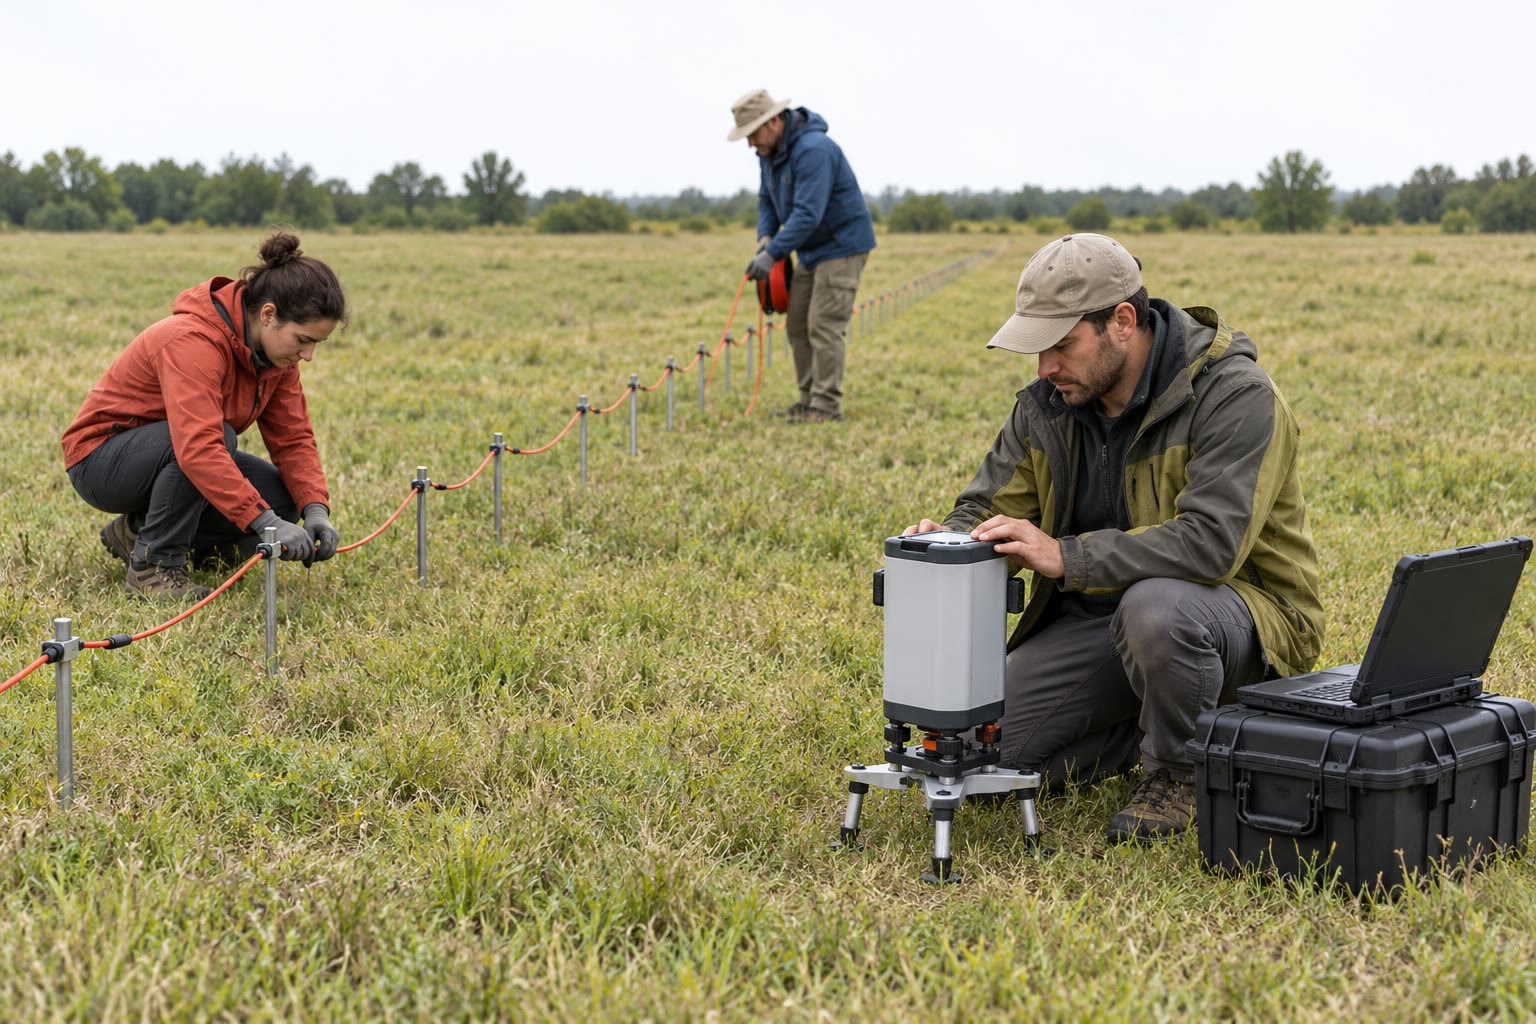
\includegraphics[width=\linewidth]{images/book5/ai/b3-geophysics-crew.jpg}

{\scriptsize يمدّ طاقم جيوفيزيائي كابل المقاومية، ومعه
مقياس الجاذبية على قاعدته (رسم توضيحي مولَّد بالذكاء الاصطناعي).}
\end{minipage}
\end{inthefield}

\begin{example}[مسح فاردن]\label{ex:b3:field-lab-methods-3:varden}
تُظهر خريطة الجاذبية انخفاضًا مغلقًا بنحو \qty{-2.3}{\milli\gal}
مركزه في الغرانيت، ممتدّ شمال--جنوب: فالغرانيت الخفيف
يمتدّ تحت الغطاء، وأطول ما يكون في ذلك الاتجاه. ويمتدّ الانخفاض
نحو \qty{1}{km} من الانكشاف، لذا يتّسع الجسم مع
العمق. ويعطي نصف عرضه عمقًا أوّليًا لكرة مكافئة؛
وتُظهر نماذج لها جانب رأسي وقاع أنّ قاعًا يقع بين واحد
وعدّة كيلومترات في العمق يفسّر القمّة بالقدر نفسه، ضمن بضعة
أعشار من المليغال، فيبقى القاع مجهولًا---وهو اللاوحدانية في
القسم السابق. وعلى قاع الوادي فوق الغرانيت، يبدأ السبر
عند مقاومية الحصى الجاف، ويهبط حيث
يدخل التيار الرواسب الغرينية المشبعة بالماء، ثم يرتفع على طول خط مستقيم
ميله واحد: غطاء ناقل فوق قاعدة شديدة المقاومية، هي
الغرانيت، على عمق بضعة أمتار. ويُظهر الرادار المجرور على القاع نفسه
صدًى مستويًا عند نحو \qty{20}{ns}: منسوب المياه الجوفية. أمّا الخطّ المغناطيسي
عبر الجناح الغربي للطية، حيث الغطاء سميك ويقع الشيست القاعدي
على عمق مئتي متر تقريبًا، ويسجّل
ذروةً متناظرة بمقدار نحو \qty{20}{nT} لا تفسّرها أيّ خريطة: قاطعًا مافيًا
غنيًا بالمغنتيت، مطمورًا تحت الغطاء؛ وامتداده على طول
خط الزوال المغناطيسي هو سبب تناظر الشذوذ. ويصف الجيوفيزيائيون
ذلك بأنّه قاطع من الدولوريت ينقطع عند عدم التوافق، والذي
يُخفيه غطاء الخريطة. وتختزل مسألة نهاية الأسبوع بيانات
المسح.
\end{example}
% ledger: gpg:susceptibility, gpg:resistivity, gpg:gpr-table

\section{التمارين}

\begin{exercise}[$\star$]\label{exo:b3:field-lab-methods-3:1}
(أ)~ما الكسر من $g = \qty{9.81}{m.s^{-2}}$ الذي تمثّله \qty{0.01}{\milli\gal}؟
(ب)~بأيّ مقدار يجب رفع مقياس الجاذبية حتى تتغيّر قراءته
بمقدار \qty{0.01}{\milli\gal} بتأثير الهواء الحر وحده؟ (ج)~بتأثير
الهواء الحر وبوغير معًا، عند كثافة
\qty{2670}{kg.m^{-3}}؟
\end{exercise}

\begin{exercise}[$\star$]\label{exo:b3:field-lab-methods-3:2}
كرة نصف قطرها \qty{50}{m} وتباين كثافتها
\qty{+500}{kg.m^{-3}} ومركزها على عمق \qty{100}{m}. احسب
الكتلة الفائضة، وذروة شذوذها، ونصف عرضه $x_{1/2}$.
\end{exercise}

\begin{exercise}[$\star$]\label{exo:b3:field-lab-methods-3:3}
ترتيب ونر ذو التباعد $a = \qty{10}{m}$ يحقن \qty{0.1}{A}
ويقيس \qty{0.239}{V}. (أ)~احسب العامل الهندسي
\omterm{def:b3:field-lab-methods-3:resistivity}{والمقاومية الظاهرية}. (ب)~بيّن أنّ ترتيب شلمبرجر الذي فيه $s =
\qty{15}{m}$ و$l = \qty{5}{m}$ له العامل الهندسي نفسه،
واشرح السبب.
\end{exercise}

\begin{exercise}[$\star$]\label{exo:b3:field-lab-methods-3:4}
للغرانيت $\varepsilon_r = 5$. (أ)~احسب سرعة الرادار. (ب)~يقع
كسر على عمق \qty{10}{m}: احسب زمن الذهاب والإياب لصداه.
(ج)~مع $\sigma = \qty{1}{mS.m^{-1}}$، احسب عمق الاختراق
والعمق المفيد، أي نحو ثلاثة أعماق اختراق. (د)~قارن مع طين رطب
ذي $\varepsilon_r = 20$ و$\sigma = \qty{10}{mS.m^{-1}}$.
\end{exercise}

\begin{exercise}[$\star\star$]\label{exo:b3:field-lab-methods-3:5}
(أ)~استنتج شذوذ أسطوانة أفقية طويلة نصف قطرها $R$ وتباين
كثافتها $\Delta\rho$، ومحورها على عمق $z$، انطلاقًا من شذوذ
كتلة خطّية، وبيّن أنّ $z = x_{1/2}$. (ب)~تعطي أسطوانة وكرة
الذروة نفسها ونصف العرض نفسه $x_{1/2} = \qty{100}{m}$.
قارن عمقيهما. أيّ التفسيرين يعطي الجسم الأعمق؟
\end{exercise}

\begin{exercise}[$\star\star$]\label{exo:b3:field-lab-methods-3:6}
شذوذ بوغير لنموذج غرانيت فاردن، مأخوذًا كلّ
\qty{100}{m} على خريطة من \num{1120} نقطة تغطّي $\qty{3.5}{km}
\times \qty{3.2}{km}$، ومجموعه \qty{-438}{\milli\gal}. (أ)~احسب
عجز الكتلة بتطبيق \cref{prop:b3:field-lab-methods-3:gauss}.
(ب)~عجز كتلة النموذج هو \qty{1.74e11}{kg}. ما الكسر الذي
تستعيده الخريطة، وأين يقع الباقي؟
\end{exercise}

\begin{exercise}[$\star\star$]\label{exo:b3:field-lab-methods-3:7}
(أ)~لقاطع رقيق قمّته على عمق \qty{30}{m}. باستعمال قاعدة الثلاث
قراءات لكلّ نصف عرض، حيث نصف العرض هو العرض الكامل للشذوذ عند نصف
ذروته، ما تباعد المحطات الذي يحتاجه؟ (ب)~والأمر نفسه
لقمّة على عمق \qty{220}{m}. (ج)~لماذا لا يستطيع مسح واحد
تمييز الجسمين الضحل والعميق معًا إلّا إذا صُمّم المسح لأجل
الضحل؟
\end{exercise}

\begin{exercise}[$\star\star$]\label{exo:b3:field-lab-methods-3:8}
حجر رملي مشبع بماء مقاومته \qty{8}{\ohm\metre} له مقاومة
تساوي \qty{80}{\ohm\metre}. (أ)~مع $a = 1$ و$m = 2$،
احسب مسامّيته. (ب)~كرّر مع $m = 1.8$ و$m = 2.2$. أيّ
حدّ في القياس يتحكّم في عدم اليقين في المسامية؟
\end{exercise}

\begin{exercise}[$\star\star$]\label{exo:b3:field-lab-methods-3:9}
  (أ)~احسب الحدود الثلاثة الأولى من المتسلسلة ذات الطبقتين
الواردة في \cref{prop:b3:field-lab-methods-3:layers} عند $s = 2h_1$ من أجل $k =
\num{0.5}$ و$k = \num{-0.5}$، والمقاوميات الظاهرية التي
تعطيها. (ب)~ما نهايات $\rho_a/\rho_1$ من أجل $s \ll h_1$
و$s \gg h_1$؟ (ج)~ما نسب المقاومية $\rho_2/\rho_1$ التي تناظر
$k = \pm 0.5$؟
\end{exercise}

\begin{exercise}[$\star\star\star$]\label{exo:b3:field-lab-methods-3:10}
  (أ)~استنتج العامل الهندسي لترتيب فينر من
\cref{thm:b3:field-lab-methods-3:point-source}. (ب)~استنتج العامل المناظر لترتيب
شلمبرجر، وبيّن أنّ $\rho_a \to 2\pi s^2(-\mathrm{d}V/
\mathrm{d}r)/I$ عندما $l/s \to 0$. (ج)~بكم يبالغ العامل التقريبي
$\pi s^2/(2l)$ في تقدير العامل الدقيق عندما $l = s/10$؟
\end{exercise}

\begin{exercise}[$\star\star\star$]\label{exo:b3:field-lab-methods-3:11}
تقع محطة على ارتفاع \qty{50}{m} فوق القاعدة، وقراءتها دقيقة حتى
\qty{0.01}{\milli\gal}، وارتفاعها حتى \qty{5}{cm}؛ وعدم اليقين في كثافة صفيحة بوغير يبلغ
\qty{100}{kg.m^{-3}}، وفي \omterm{def:b3:field-lab-methods-3:terrain}{تصحيح التضاريس} بمقدار
\qty{0.2}{\milli\gal}. (أ)~أعدّ ميزانية الخطأ لشذوذ بوغير الخاص بها.
(ب)~أيّ حدّ يهيمن، وأيّ حدّ ينبغي تحسينه لرصد شذوذ
قدره \qty{0.1}{\milli\gal}؟ (ج)~ما المجموع من دون
حدّ التضاريس؟
\end{exercise}

\begin{exercise}[$\star\star\star$]\label{exo:b3:field-lab-methods-3:12}
قراءات الجاذبية الخمس عبر جسم مدفون، عند $x = -600$، $-300$، $0$،
$300$ و\qty{600}{m}، هي \num{-0.69}، \num{-2.17}، \num{-4.16}،
\num{-2.10} و\qty{-0.73}{\milli\gal}، كلّ منها بانحراف معياري $\sigma =
\qty{0.03}{\milli\gal}$. (أ)~بالنسبة إلى نماذج الكرة المتمركزة تحت $x = 0$ على أعماق
\num{300}، \num{400} و\qty{500}{m}، اختر الكتلة التي تطابق
القراءة المركزية، واحسب مربّع \omterm{def:b3:field-lab-methods-3:inversion-practice}{عدم التطابق} $\chi^2$ لكلّ منها. (ب)~أيّ
نموذج يطابق البيانات ضمن أخطائها؟ (ج)~هل يمكن لجسم بشكل آخر
يطابقها بالقدر نفسه؟ ما الذي سيحسم الأمر؟
\end{exercise}

\section{مسألة: الأجسام المخفية في تلال فاردن}

\begin{problem}[{مسألة نهاية الأسبوع --- اختزال مسح فاردن}]
\label{pb:b3:field-lab-methods-3:1}
استخدم $G = \qty{6.674e-11}{m^3.kg^{-1}.s^{-2}}$، وتدرّج الهواء الحر
\qty{0.3086}{\milli\gal.m^{-1}}، ومعامل بوغير
\qty{0.1119}{\milli\gal.m^{-1}} (الكثافة \qty{2670}{kg.m^{-3}}).

\medskip\noindent\textbf{الجزء الأول --- حلقة الجاذبية.} تُعطي الحلقة على
المقطع الجاذبي القراءات (بالمليغال بعد المعايرة، والارتفاعات بالمتر،
والأزمنة بالساعات بعد الساعة 09:00):
\begin{center}
\small
\begin{tabular}{lccccc}
\hline
المحطة & القاعدة & \qty{3.0}{km} & \qty{3.5}{km} & \qty{4.0}{km} & القاعدة \\
\hline
الزمن & 0 & 0.5 & 0.9 & 1.3 & 2.0 \\
الارتفاع & 176.1 & 149.0 & 145.5 & 158.0 & 176.1 \\
القراءة & 2846.512 & 2851.075 & 2850.497 & 2849.392 & 2846.708 \\
\hline
\end{tabular}
\end{center}
\begin{enumerate}
\item احسب معدّل انجراف الحلقة.
\item صحّح قراءات المحطات الثلاث من أجل الانجراف، وعبّر عنها
  بالنسبة إلى القاعدة.
\item طبّق تصحيحي الهواء الحر وبوغير لفروق الارتفاع،
  واحسب شذوذ بوغير لكلّ محطة بالنسبة إلى
  القاعدة.
\item كان \omterm{def:b3:field-lab-methods-3:gravimeter}{الانجراف الآلي} وحده \qty{0.040}{\milli\gal.h^{-1}}.
  ما الذي سبّب بقية التغيّر عند القاعدة، ولماذا يمكن
  إزالته مع الانجراف؟
\item يعطي النموذج الذي أُخذت منه القراءات الشذوذات الثلاثة
  بالنسبة إلى القاعدة: \num{-0.825}، \num{-2.131}
  و\qty{-0.825}{\milli\gal}. احسب أخطاء الاختزال. والارتفاعات
  في الجدول مُقرَّبة إلى \qty{0.1}{m}: ما الخطأ الذي يمكن أن يُدخله
  هذا التقريب، وهل يفسّر ذلك الأخطاء؟
\item ما دقّة الارتفاع التي تُبقي الشذوذ المختزل ضمن
  \qty{0.01}{\milli\gal}؟ لماذا تطلب أدلّة المسح
  \qty{3.3}{cm}، وهو رقم أكثر صرامة؟
\end{enumerate}

\medskip\noindent\textbf{الجزء الثاني --- شذوذ الغرانيت.} على طول
المقطع يبلغ الشذوذ أدنى قيمة له، \qty{-2.293}{\milli\gal}، عند
$x = \qty{3.50}{km}$، ويمرّ بنصف تلك القيمة عند $x = 3.048$
و\qty{3.952}{km}. يملك نموذج الغرانيت تباينًا في الكثافة مقداره
\qty{-130}{kg.m^{-3}}، وسطح الأرض عند المركز على ارتفاع \qty{145.5}{m}
فوق مستوى سطح البحر.
\begin{enumerate}[resume]
\item احسب نصف العرض $x_{1/2}$ وعمق مركز
  الكرة المكافئة.
\item احسب عجز كتلة تلك الكرة، ونصف قطرها من أجل
  تباين الكثافة للغرانيت. ما الغريب في النتيجة؟
\item يبلغ مركز كتلة النموذج \qty{864}{m} تحت سطح الأرض، وعجز كتلته
  \qty{1.74e11}{kg}. لماذا تعطي قاعدة نصف العرض جسمًا
  أقلّ عمقًا وأخفّ كتلةً؟
\item أسطوانة رأسية لها المساحة نفسها للغرانيت عند
  عدم التوافق ونصف قطرها \qty{461}{m}. احسب شذوذها على المحور
  من أجل قمّة عند سطح الأرض وقاع عند عمق \qty{1645}{m}، ومن أجل
  عمق غير محدود.
\item أوجد، بالتجربة أو بالحل، عمق القاع الذي تعطي عنده هذه
  الأسطوانة الشذوذ المرصود \qty{-2.29}{\milli\gal}.
\item احسب شذوذ الأسطوانة وقمّتها على عمق \qty{6}{m}
  (القاع \qty{1645}{m}). هل تستطيع الجاذبية أن تبيّن ما إذا كان الغرانيت يصل
  إلى السطح تحت الرواسب الفيضية؟
\end{enumerate}

\medskip\noindent\textbf{الجزء الثالث --- قاع الوادي.} يُعطي السبر الكهربائي بترتيب
شلمبرجر على القاع فوق الغرانيت (نصف المسافة $s$
بالأمتار، $\rho_a$ بوحدة \unit{\ohm\metre}):
\begin{center}
\small
\begin{tabular}{lcccccccc}
\hline
$s$ & 1 & 2 & 4 & 6 & 10 & 20 & 30 & 40 \\
$\rho_a$ & 577 & 526 & 387 & 350 & 449 & 821 & 1309 & 1684 \\
\hline
\end{tabular}
\end{center}
على مقطع راداري على امتداد القاع نفسه، يعطي أنبوبٌ قطعًا زائدًا قمّته
عند \qty{10.7}{ns}، وزمنًا قدره \qty{17.1}{ns} على بُعد \qty{1}{m}
جانبًا؛ ويصل صدًى مسطّح عند \qty{20.0}{ns}.
\begin{enumerate}[resume]
\item عند $s = \qty{20}{m}$ كان طول MN هو \qty{2}{m}، وكان التيار
  \qty{50}{mA}. احسب العامل الهندسي وفرق الجهد المقيس.
\item احسب سرعة الرادار، والسماحية النسبية للرواسب
  الفيضية وعمق الأنبوب.
\item الصدى المسطّح هو منسوب المياه الجوفية. ما عمقه؟
\item قدّر الموصلية $S$ للرواسب الفيضية من القراءات عند
  20، 30 و\qty{40}{m}.
\item للرواسب الفيضية الجافة مقاومية \qty{600}{\ohm\metre}، وللرواسب الفيضية
  المشبعة \qty{222}{\ohm\metre}. احسب سمك الطبقة المشبعة
  من الرواسب الفيضية وعمق قمّة الغرانيت. هل التقدير مرتفع
  أم منخفض، ولماذا؟
\item مقاومية المياه الجوفية \qty{20}{\ohm\metre}. احسب مسامية
  الرواسب الفيضية \omterm{prop:b3:field-lab-methods-3:archie}{بقانون آرتشي} عند $m = 2$، ومدى $m$
  بين \num{1.3} و\num{2.8}.
\end{enumerate}

\medskip\noindent\textbf{الجزء الرابع --- الخط المغناطيسي.} يمتدّ الخط
شرقًا من $x = \qty{1.70}{km}$، محطة كل \qty{50}{m} وكل
دقيقتين؛ وسجّلت محطة القاعدة في الدقائق نفسها. أمّا
القراءات، بعد طرح \qty{48000}{nT}، فهي:
\begin{center}
\small
\setlength{\tabcolsep}{3.5pt}
\begin{tabular}{lccccccccccc}
\hline
$x$ (كم) & 1.70 & 1.75 & 1.80 & 1.85 & 1.90 & 1.95 & 2.00 & 2.05 & 2.10 & 2.15 & 2.20 \\
الخط & 3.4 & 4.8 & 6.3 & 8.1 & 10.3 & 12.8 & 15.8 & 19.2 & 22.9 & 26.2 & 28.0 \\
القاعدة & 0.0 & 0.7 & 1.5 & 2.2 & 2.9 & 3.6 & 4.3 & 5.0 & 5.7 & 6.4 & 7.0 \\
\hline
$x$ (كم) & 2.25 & 2.30 & 2.35 & 2.40 & 2.45 & 2.50 & 2.55 & 2.60 & 2.65 & 2.70 & \\
الخط & 27.7 & 25.8 & 23.3 & 20.9 & 19.0 & 17.6 & 16.6 & 15.9 & 15.5 & 15.2 & \\
القاعدة & 7.6 & 8.2 & 8.8 & 9.4 & 9.9 & 10.4 & 10.9 & 11.3 & 11.7 & 12.1 & \\
\hline
\end{tabular}
\end{center}
المجال الرئيسي يبلغ \qty{48000}{nT}، ويميل بزاوية \ang{65}.
\begin{enumerate}[resume]
\item طبّق \omterm{def:b3:field-lab-methods-3:magnetic}{التصحيح اليومي}، وأعطِ الشذوذ المصحَّح عند
  كل محطة.
\item بيّن أنّه بدون التصحيح لا ينخفض الشذوذ أبدًا إلى نصف
  قمّته على الجانب الشرقي.
\item حدّد القمّة والنقطتين اللتين يساوي فيهما الشذوذ المصحَّح
  نصف القمّة بالاستيفاء الخطي، واحسب نصف العرض.
\item الشذوذ متناظر. ماذا يدلّ ذلك على امتداد
  الجسم، وأيّ نوع من الأجسام تفترضه قاعدة نصف العرض؟
\item احسب الجداء $\kappa t$ للقابلية المغناطيسية والسماكة.
  إذا كان القاطع دولريتًا قابليته المغناطيسية \num{0.03}، فما مقدار
  سماكته؟
\item هل كانت المحطات متقاربة بما يكفي؟
\item أعطِ عمق قمّة القاطع المدفون تحت سطح الأرض، مقرّبًا
  إلى أقرب عشرة أمتار، وقارنه بعمق
  عدم التوافق في النموذج الجيولوجي للمنطقة، البالغ \qty{222}{m} عند هذه
  النقطة.
\end{enumerate}
\end{problem}
% ledger: gpg:grav-survey, gpg:mag-field, keys:archie
